% Options for packages loaded elsewhere
\PassOptionsToPackage{unicode}{hyperref}
\PassOptionsToPackage{hyphens}{url}
\PassOptionsToPackage{dvipsnames,svgnames,x11names}{xcolor}
%
\documentclass[
]{article}

\usepackage{amsmath,amssymb}
\usepackage{lmodern}
\usepackage{iftex}
\ifPDFTeX
  \usepackage[T1]{fontenc}
  \usepackage[utf8]{inputenc}
  \usepackage{textcomp} % provide euro and other symbols
\else % if luatex or xetex
  \usepackage{unicode-math}
  \defaultfontfeatures{Scale=MatchLowercase}
  \defaultfontfeatures[\rmfamily]{Ligatures=TeX,Scale=1}
\fi
% Use upquote if available, for straight quotes in verbatim environments
\IfFileExists{upquote.sty}{\usepackage{upquote}}{}
\IfFileExists{microtype.sty}{% use microtype if available
  \usepackage[]{microtype}
  \UseMicrotypeSet[protrusion]{basicmath} % disable protrusion for tt fonts
}{}
\makeatletter
\@ifundefined{KOMAClassName}{% if non-KOMA class
  \IfFileExists{parskip.sty}{%
    \usepackage{parskip}
  }{% else
    \setlength{\parindent}{0pt}
    \setlength{\parskip}{6pt plus 2pt minus 1pt}}
}{% if KOMA class
  \KOMAoptions{parskip=half}}
\makeatother
\usepackage{xcolor}
\setlength{\emergencystretch}{3em} % prevent overfull lines
\setcounter{secnumdepth}{5}
% Make \paragraph and \subparagraph free-standing
\ifx\paragraph\undefined\else
  \let\oldparagraph\paragraph
  \renewcommand{\paragraph}[1]{\oldparagraph{#1}\mbox{}}
\fi
\ifx\subparagraph\undefined\else
  \let\oldsubparagraph\subparagraph
  \renewcommand{\subparagraph}[1]{\oldsubparagraph{#1}\mbox{}}
\fi


\providecommand{\tightlist}{%
  \setlength{\itemsep}{0pt}\setlength{\parskip}{0pt}}\usepackage{longtable,booktabs,array}
\usepackage{calc} % for calculating minipage widths
% Correct order of tables after \paragraph or \subparagraph
\usepackage{etoolbox}
\makeatletter
\patchcmd\longtable{\par}{\if@noskipsec\mbox{}\fi\par}{}{}
\makeatother
% Allow footnotes in longtable head/foot
\IfFileExists{footnotehyper.sty}{\usepackage{footnotehyper}}{\usepackage{footnote}}
\makesavenoteenv{longtable}
\usepackage{graphicx}
\makeatletter
\def\maxwidth{\ifdim\Gin@nat@width>\linewidth\linewidth\else\Gin@nat@width\fi}
\def\maxheight{\ifdim\Gin@nat@height>\textheight\textheight\else\Gin@nat@height\fi}
\makeatother
% Scale images if necessary, so that they will not overflow the page
% margins by default, and it is still possible to overwrite the defaults
% using explicit options in \includegraphics[width, height, ...]{}
\setkeys{Gin}{width=\maxwidth,height=\maxheight,keepaspectratio}
% Set default figure placement to htbp
\makeatletter
\def\fps@figure{htbp}
\makeatother
\newlength{\cslhangindent}
\setlength{\cslhangindent}{1.5em}
\newlength{\csllabelwidth}
\setlength{\csllabelwidth}{3em}
\newlength{\cslentryspacingunit} % times entry-spacing
\setlength{\cslentryspacingunit}{\parskip}
\newenvironment{CSLReferences}[2] % #1 hanging-ident, #2 entry spacing
 {% don't indent paragraphs
  \setlength{\parindent}{0pt}
  % turn on hanging indent if param 1 is 1
  \ifodd #1
  \let\oldpar\par
  \def\par{\hangindent=\cslhangindent\oldpar}
  \fi
  % set entry spacing
  \setlength{\parskip}{#2\cslentryspacingunit}
 }%
 {}
\usepackage{calc}
\newcommand{\CSLBlock}[1]{#1\hfill\break}
\newcommand{\CSLLeftMargin}[1]{\parbox[t]{\csllabelwidth}{#1}}
\newcommand{\CSLRightInline}[1]{\parbox[t]{\linewidth - \csllabelwidth}{#1}\break}
\newcommand{\CSLIndent}[1]{\hspace{\cslhangindent}#1}

\usepackage{arxiv}
\usepackage{orcidlink}
\usepackage{amsmath}
\usepackage[T1]{fontenc}
\makeatletter
\makeatother
\makeatletter
\makeatother
\makeatletter
\@ifpackageloaded{caption}{}{\usepackage{caption}}
\AtBeginDocument{%
\ifdefined\contentsname
  \renewcommand*\contentsname{Table of contents}
\else
  \newcommand\contentsname{Table of contents}
\fi
\ifdefined\listfigurename
  \renewcommand*\listfigurename{List of Figures}
\else
  \newcommand\listfigurename{List of Figures}
\fi
\ifdefined\listtablename
  \renewcommand*\listtablename{List of Tables}
\else
  \newcommand\listtablename{List of Tables}
\fi
\ifdefined\figurename
  \renewcommand*\figurename{Figure}
\else
  \newcommand\figurename{Figure}
\fi
\ifdefined\tablename
  \renewcommand*\tablename{Table}
\else
  \newcommand\tablename{Table}
\fi
}
\@ifpackageloaded{float}{}{\usepackage{float}}
\floatstyle{ruled}
\@ifundefined{c@chapter}{\newfloat{codelisting}{h}{lop}}{\newfloat{codelisting}{h}{lop}[chapter]}
\floatname{codelisting}{Listing}
\newcommand*\listoflistings{\listof{codelisting}{List of Listings}}
\makeatother
\makeatletter
\@ifpackageloaded{caption}{}{\usepackage{caption}}
\@ifpackageloaded{subcaption}{}{\usepackage{subcaption}}
\makeatother
\makeatletter
\@ifpackageloaded{tcolorbox}{}{\usepackage[many]{tcolorbox}}
\makeatother
\makeatletter
\@ifundefined{shadecolor}{\definecolor{shadecolor}{rgb}{.97, .97, .97}}
\makeatother
\makeatletter
\makeatother
\ifLuaTeX
  \usepackage{selnolig}  % disable illegal ligatures
\fi
\IfFileExists{bookmark.sty}{\usepackage{bookmark}}{\usepackage{hyperref}}
\IfFileExists{xurl.sty}{\usepackage{xurl}}{} % add URL line breaks if available
\urlstyle{same} % disable monospaced font for URLs
\hypersetup{
  pdftitle={They're Clutching up! Team Momentum in Round-Based Esports},
  pdfauthor={Tony ElHabr},
  colorlinks=true,
  linkcolor={blue},
  filecolor={Maroon},
  citecolor={Blue},
  urlcolor={Blue},
  pdfcreator={LaTeX via pandoc}}

\title{They're Clutching up! Team Momentum in Round-Based Esports}
\author{
Tony ElHabr\\\\Georgia Institute of
Technology\\\\\href{mailto:anthonyelhabr@gmail.com}{anthonyelhabr@gmail.com}}
\date{}
\begin{document}
\maketitle
\begin{abstract}
My research investigates patterns in round win percentages in
professional Search and Destroy (SnD) matches of the popular
first-person shooter game Call of Duty (CoD).

First, I find evidence in CoD defying the naive hypothesis that a series
represents a sequence of independent events (rounds), with each team
having a constant 50\% probability of winning a given round.

Second, I examine post-streak round win probability. I find that teams
perform significantly worse than expected after streaks of 2, 3, and 4
wins when series end up going to 9, 10, or 11 (maximum) rounds, even
after accounting for the ``hot-hand'' phenomenon.

Third, I compare win percentages in round one versus all other rounds,
hypothesizing that there may be some advantage on either side when there
is no prior information about how the opponent intends to play a given
map in either game. I find only one instance for which there seems to be
a significant defensive advantage in round one.

Finally, I evaluate behavior when teams have two rounds left to win the
series, observing a peak in COD offensive win percentages in the 4-4
state, and no such oddity in Valorant.
\end{abstract}
\ifdefined\Shaded\renewenvironment{Shaded}{\begin{tcolorbox}[interior hidden, enhanced, boxrule=0pt, borderline west={3pt}{0pt}{shadecolor}, sharp corners, frame hidden, breakable]}{\end{tcolorbox}}\fi

\hypertarget{introduction}{%
\section{Introduction}\label{introduction}}

\hypertarget{description-of-call-of-duty-search-and-destroy}{%
\subsection{1 Description of Call of Duty Search and
Destroy}\label{description-of-call-of-duty-search-and-destroy}}

Call of Duty (CoD), first released in 2003, is one of the most popular
first-person shooter (FPS) video game franchises of all-time. Tthe most
popular mode in the competitive scene is ``Search and Destroy'' (SnD),
which bears resemblance to ``Bomb Defusal'' in Counter-Strike and
``Plant/Defuse'' in Valorant, two other FPS games played in professional
leagues. SnD is one-sided game mode in which one team, the offensive
side, tries to destroy one of two designated bomb sites on the map.

In professional CoD, a team must win six rounds of SnD to win the
match.\footnote{A maximum of 11 even rounds can be played. There is no
  ``sudden death'' or ``win by two'' rule like there are for SnD
  equivalent in professional Counter-Strike and Valorant matches.} A
round can end in one of four ways:

\begin{enumerate}
\def\labelenumi{\arabic{enumi}.}
\tightlist
\item
  One team eliminates all members of the other team prior to a bomb
  plant. (Eliminating team wins.)
\item
  The offensive team eliminates all members of the defensive team after
  a bomb plant.\footnote{\begin{itemize}
    \tightlist
    \item
      The bomb can be picked up by any member of the offensive team.
    \item
      The bomb carrier is not obstructed at all by carrying the bomb
      (i.e.~movement is the same, weapon usage is the same).
    \item
      The defense does not get any visual indication for who is carrying
      the bomb.
    \item
      A bomb plant takes five seconds. The timer resets if the player
      stops planting site prior to completing it.
    \item
      A bomb defuse takes seven seconds. The timer resets if the player
      ``drops'' the bomb.
    \item
      The bomb takes 45 seconds to defuse after being planted.
    \end{itemize}} (Offense wins.)
\item
  The defensive team defuses the bomb after a bomb plant.\footnote{Often
    the defensive team will try to eliminate all team members prior to
    making the defuse, but in some cases, they may try to ``ninja''
    defuse.} (Defense wins.)
\item
  The offensive team does not make a plant by the time the round timer
  ends. (Defense wins.)
\end{enumerate}

Teams take turns playing offense and defense every round.

\hypertarget{data}{%
\subsection{1. Data}\label{data}}

CoD has roughly gone through three eras of professional gaming: (1)
Major League Gaming (MLG) tournaments prior to 2016; (2) the CoD World
League (CWL), initiated in 2016; and (3) the 12-franchise CoD League
(CDL), running since 2020 and completing three year-long ``seasons''
completed as of August 2022.\footnote{CoD is fairly unique compared to
  other esports in that it runs on an annual lifecycle (released coming
  in the late fall), where a new game is published every year under the
  same title. Each new game bears resemblance to past ones, often
  introducing relatively small variations (``improvements'') to
  graphics, game modes, and other facets of gameplay. During the CDL
  era, the games released have been Modern Warfare (2020), Cold War
  (2021) and Vanguard (2022).} The data set consists of all SnD matches
played in tournaments and qualifiers during the CDL era, totaling 1,704
series played, in which there were 15,584 rounds played. Data was
collected in spreadsheets by community member ``IOUTurtle''.\footnote{Data:
  https://linktr.ee/CDLArchive. Author: https://twitter.com/IOUTurtle}

I adopt the terminology ``series'' to refer to what CoD SnD players
typically call a ``match'', so as to emulate the terminology of playoff
series in professional leagues like the National Basketball Association,
National Hockey League, and Major League Baseball. A ``game'' or a
``match'' in such leagues is analogous to a ``round'' of CoD SnD.

\hypertarget{literature-review}{%
\section{Literature review}\label{literature-review}}

There have been only a handful of studies of the distribution of games
played in a series, most of which assume a constant probability \(p\) of
a given team winning a game in the series, regardless of the series
state. Observing that the American League had dominated the National
League in Major League Baseball's (MLB) World Series matchups, implying
that matchups should not modeled with \(p=0.5\), (Mosteller 1952)
proposed three approaches for identifying the optimal constant
probability value of the stronger team in the World Series, finding
\(p \approx 0.65\) in each case: (1) a ``method of moments'', an
approach that solves for \(p\) from the empirical average number of
games won by the loser of the series; (2) maximum likelihood, and (3)
maximum chi-square approach. (Chance 2020) re-examines the constant
probability notion in Major League Baseball's World Series (1923--2018),
the National Basketball Association's Finals (1951--2018), and the
National Hockey League's Stanley Cup (1939--2018). Chance applies
Mosteller's method 1 and 2 and finds strong evidence against the null
hypothesis of \(p = 0.5\) in the MLB and NHL championship series. Chance
outlines a conditional probability framework (likelihood of winning a
game given the series state) which can exactly explain the distribution
of the number of games played.

Momentum is one of the most frequently published topics in sports
analytics. We often use use ``streaks'' and momentum interchangeably,
but as (Steeger, Dulin, and Gonzalez 2021) note, momentum implies
dependence between events, whereas streaking does not. (sentence about
negative recency, hinting at ``hot hand''\ldots{} (Miller and Sanjurjo
2018) debunking findings from (Gilovich, Vallone, and Tversky 1985))

Despite the plethora of existing research on games played and momentum
in sports, these topics have yet to be investigated heavily in esports.
Work has been done to examine in-round win probability in other FPS
titles such as Counter-Strike ((Xenopoulos, Freeman, and Silva 2022))
and Valorant ((DeRover 2021)), both of which are round-based like CoD
SnD. However, research on round-level trends is sparse, perhaps because
games like Counter-Strike and Valorant both have economic aspects that
can create clear advantages on side in a given round, given how prior
rounds played out.\footnote{Additionally, both Counter-Strike and
  Valorant have overtime rules and blocked offensive/defensive roles
  (i.e.~playing either offense or defense for many consecutive rounds).}

\hypertarget{methodology-results-and-discussion}{%
\section{Methodology, results, and
discussion}\label{methodology-results-and-discussion}}

The empirical offensive round win percentage across all rounds is
47.8\%.\footnote{Offensive round win percentage has been nearly constant
  across the three games during the CDL era: MW (2020) 47.2\%, Cold War
  (2021) 47.9\%, Vanguard (2022) 48.1\%}
Figure~\ref{fig-cod-o-round-win-prop} shows that offensive round win
rate is not quite constant, although, on average, never veers more than
10\% from this global average.

\begin{figure}

{\centering 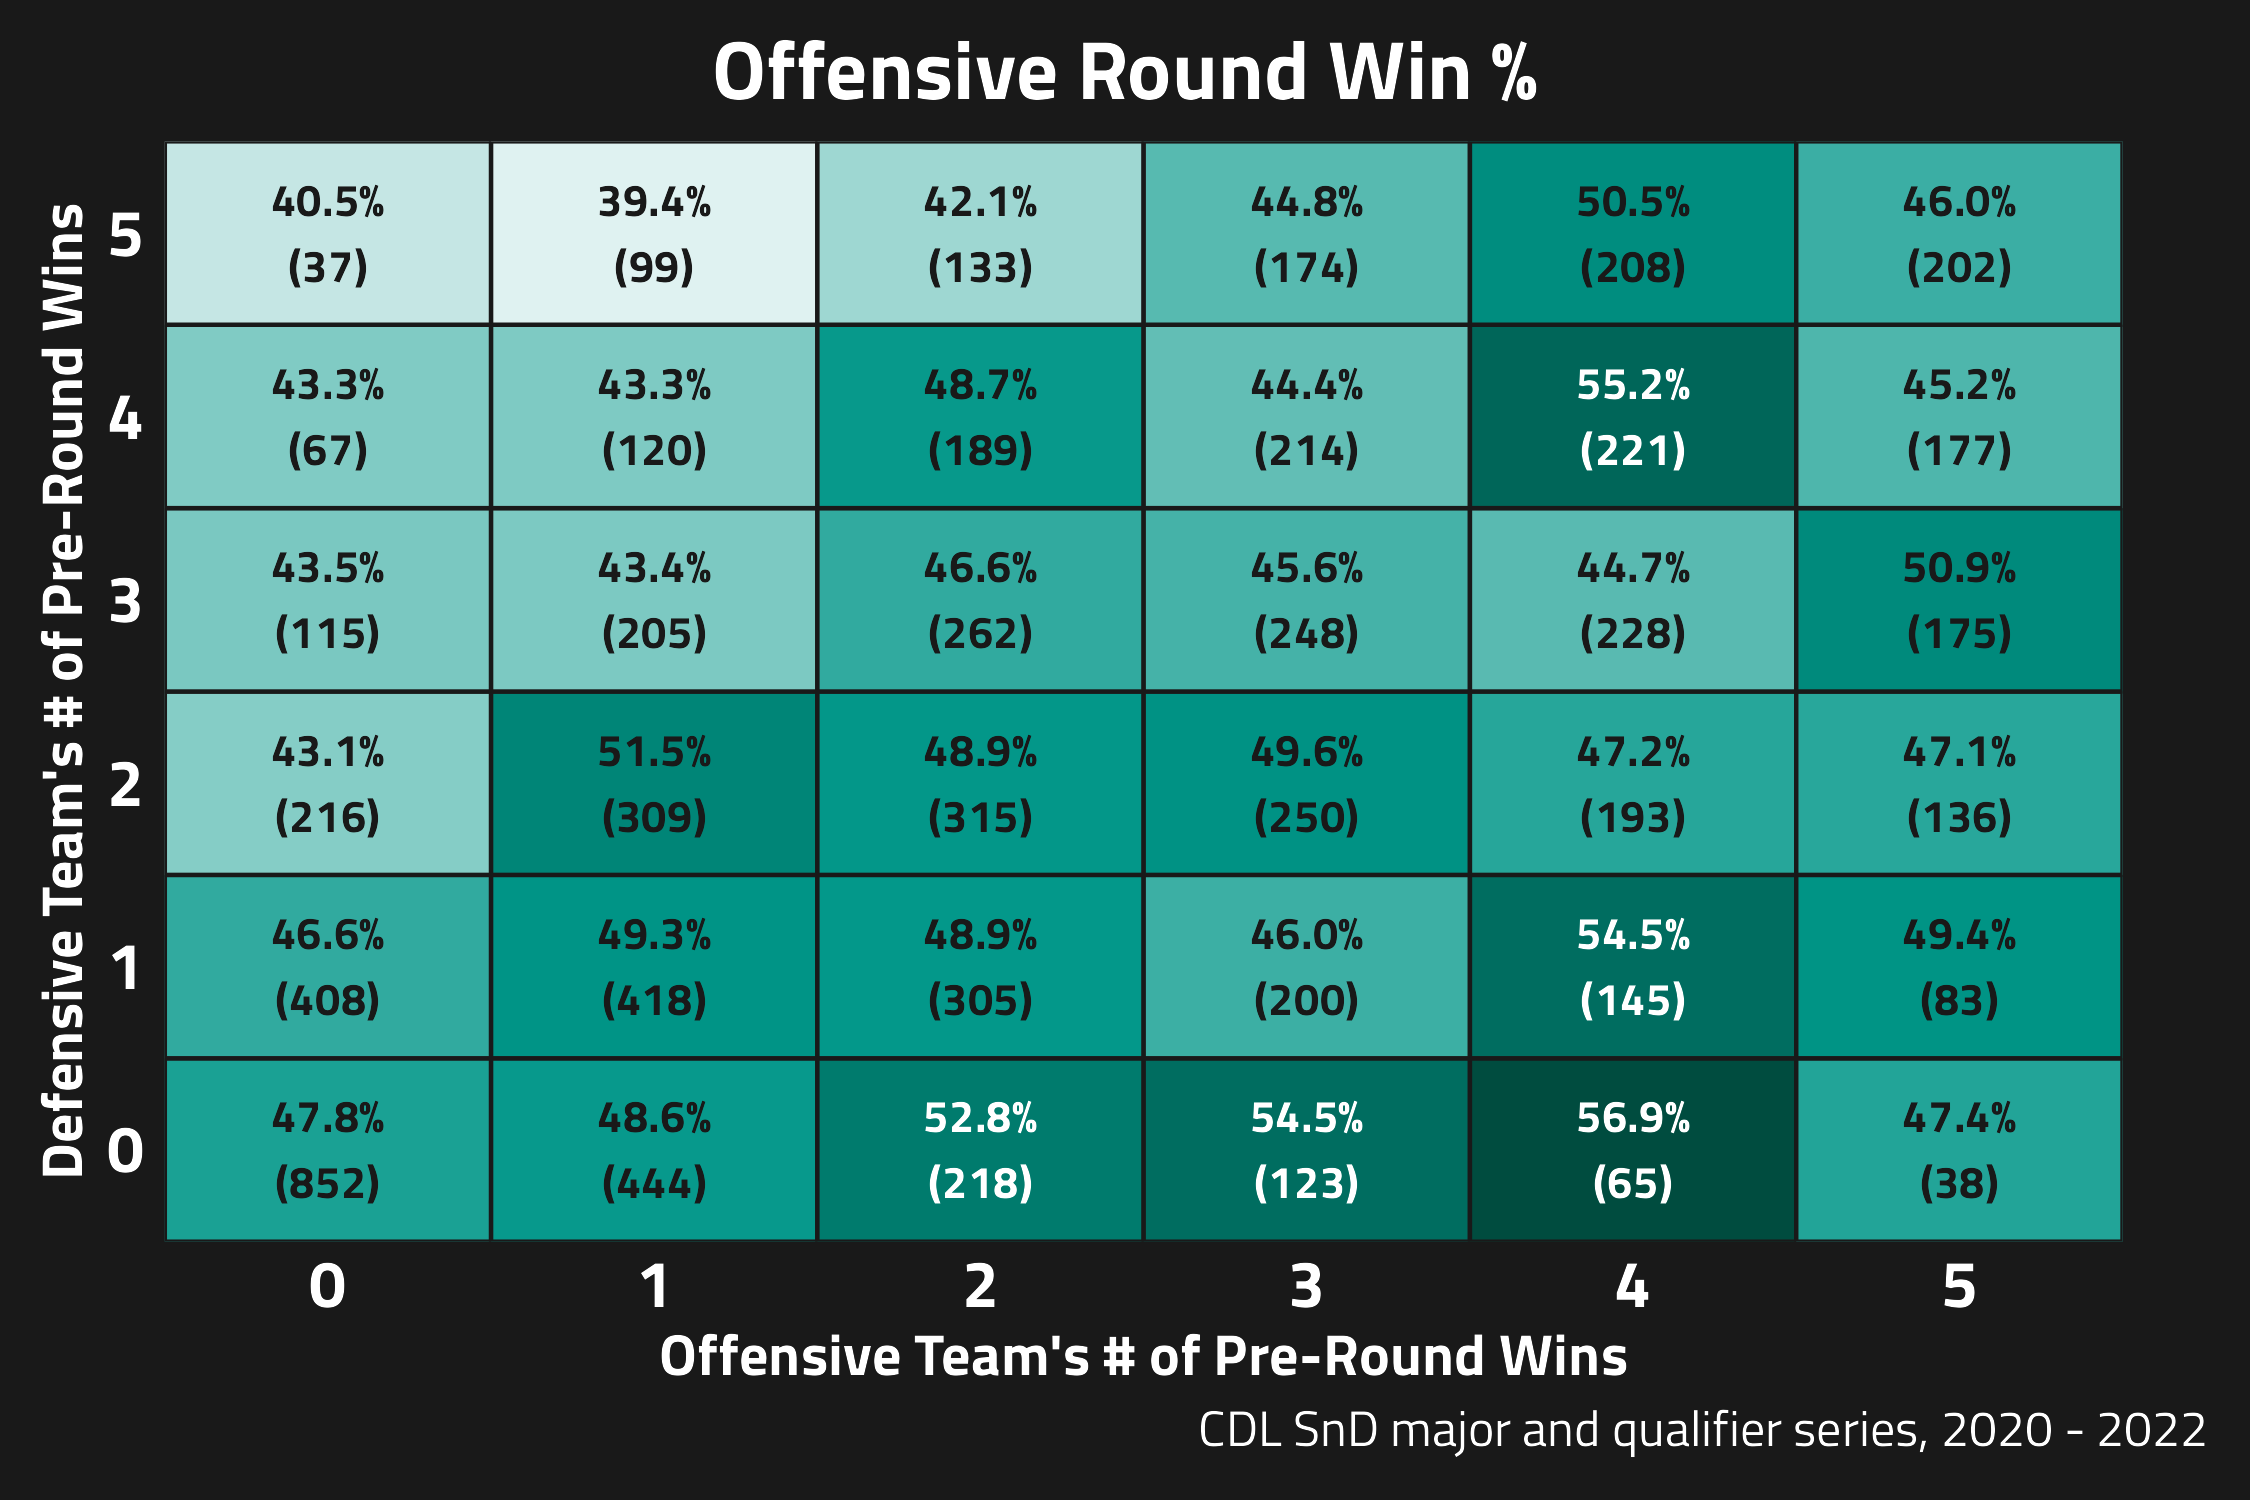
\includegraphics{images/cod_o_round_win_prop.png}

}

\caption{\label{fig-cod-o-round-win-prop}Offensive round win percentage
by series state}

\end{figure}

\hypertarget{references}{%
\section*{References}\label{references}}
\addcontentsline{toc}{section}{References}

\hypertarget{refs}{}
\begin{CSLReferences}{1}{0}
\leavevmode\vadjust pre{\hypertarget{ref-chance2020}{}}%
Chance, Don. 2020. {``Conditional Probability and the Length of a
Championship Series in Baseball, Basketball, and Hockey.''}
\emph{Journal of Sports Analytics} 6 (2): 111--27.
\url{https://doi.org/10.3233/JSA-200422}.

\leavevmode\vadjust pre{\hypertarget{ref-derover2021}{}}%
DeRover, DeMars. 2021. {``Round Win Probabilities Based on Who's Alive +
Time.''}
\url{https://www.reddit.com/r/VALORANT/comments/n3lpoo/round_win_probabilities_based_on_whos_alive_time/}.

\leavevmode\vadjust pre{\hypertarget{ref-gilovich1985}{}}%
Gilovich, Thomas, Robert Vallone, and Amos Tversky. 1985. {``The Hot
Hand in Basketball: On the Misperception of Random Sequences.''}
\emph{Cognitive Psychology} 17 (3): 295314.

\leavevmode\vadjust pre{\hypertarget{ref-miller2018}{}}%
Miller, Joshua B., and Adam Sanjurjo. 2018. {``Surprised by the Hot Hand
Fallacy? A Truth in the Law of Small Numbers.''} \emph{Econometrica} 86
(6): 20192047.

\leavevmode\vadjust pre{\hypertarget{ref-mosteller1952}{}}%
Mosteller, Frederick. 1952. {``The World Series Competition.''}
\emph{Journal of the American Statistical Association} 47 (259): 355380.

\leavevmode\vadjust pre{\hypertarget{ref-steeger2021}{}}%
Steeger, Gregory M., Johnathon L. Dulin, and Gerardo O. Gonzalez. 2021.
{``Winning and Losing Streaks in the National Hockey League: Are Teams
Experiencing Momentum or Are Games a Sequence of Random Events?''}
\emph{Journal of Quantitative Analysis in Sports} 17 (3): 155170.

\leavevmode\vadjust pre{\hypertarget{ref-xenopoulos2022}{}}%
Xenopoulos, Peter, William Robert Freeman, and Claudio Silva. 2022.
{``Analyzing the Differences Between Professional and Amateur Esports
Through Win Probability.''} In, 34183427.

\end{CSLReferences}



\end{document}
